\chapter{Dataset}
Lo studio condotto si è basato sui dati raccolti nell’ambito di un monitoraggio acustico
passivo nella \textit{Riserva Naturale Los Yátaros}, nel dipartimento di \textit{Boyacá} in \textit{Colombia} [3]. Con il termine passivo si identifica una modalità di osservazione del paesaggio incentrata sulla
registrazione di un particolare luogo e solo successivamente prevede un’analisi approfondita,
diversamente da quella attiva, dove si osserva e si analizza il fenomeno in tempo reale. La
raccolta dati è stata commissionata dalla fondazione \textit{Von Humboldt}, un ente colombiano che
si occupa di ricerca sulla biodiversità e sulle sue relazioni con il benessere umano.

La riserva è composta da querceti e foresta subandina in diversi stadi di rigenerazione
naturale, e presenta una biodiversità acustica molto particolare. Il progetto mirava a profilare
l’impronta acustica della riserva campionando suoni nello spettro udibile e negli ultrasuoni.

Sono stati predisposti tre siti, denominati \textit{YAT}, organizzati in una disposizione triangolare,
lungo il sentiero principale, distanti 150 m, con due sensori acustici \textit{AudioMoth} ciascuno, per
le due forme di suono desiderate, posti ad altezza diverse. Il periodo di campionamento si è
svolto dall’1 marzo al 2 maggio 2020, registrando un minuto di audio ad intervalli di trenta
minuti durante tutto il giorno (dalle 00:00 alle 23:30) per lo spettro dell’udibile (0 \textit{Hz} - 16 \textit{kHz}) e nella fascia notturna (dalle 16:30 alle 6:00) per lo spettro dell’ultrasuono (fino a 192 \textit{kHz}). In totale si è ottenuto 12447 registrazioni di cui 9055 nell'udibile e 3392 nell’ultrasuono. In questo progetto, sono stati considerati solo i dati nello spettro udibile, per permettere l’ascolto del contenuto.

\section{Dataset prima fase}
Nella prima fase dello studio è stato utilizzato il \textit{dataset} completo (DATA1) che presenta
l’insieme originale dei dati. Il gruppo si presenta con una suddivisione per i tre siti (YAT1,
YAT2, YAT3) con quantità leggermente differenti. Gli audio sono 3018 per \textit{yat}, a parte il
primo con 3019. Ogni sito presenta 1482 file per il mese di marzo (1483 solo per YAT1),
1440 per il mese di aprile e 96 per il mese di maggio.

Data l’ingente quantità di dati disponibile, non si è potuto analizzare il contenuto, ossia
ascoltare l’intero insieme di registrazioni. In una prima caratterizzazione, analizzando diversi
audio in momenti diversi della giornata e del mese, si è osservato che tutti e tre i luoghi 
risultano molto caratterizzati dal suono del fiume e della cascata vicina. È importante notare
che anche se tale suono fosse stato ad una distanza maggiore avrebbe sortito lo stesso effetto:
infatti Farina \textit{et al.} sostengono che “la geofonia può essere rilevata anche a grandi distanze in
base all’ampiezza della sorgente sonora” [3]. A questo si aggiungono ulteriori problematiche
dovute a periodi piovosi, il cui rumore sovrasta in diverse occasioni i suoni ambientali
naturali. Entrambi gli elementi appena descritti determinano un ambiente umido che potrebbe
influire anche sulla capacità del sensore.


\section{Dataset seconda e terza fase}
Il \textit{dataset} della seconda e terza fase dello studio (DATA2) consiste in un sottoinsieme del
\textit{dataset} DATA1. Per potere inferire maggiori informazioni dal contesto si è stabilito che era
necessaria una descrizione più accurata del contenuto. Quindi si è ristretto l’insieme ad un
campione di dati minore che potesse essere ascoltato e studiato nel dettaglio. L’analisi ha
estratto dal \textit{dataset} originale 186 audio, focalizzandosi sul sito YAT1, nel mese di marzo con
finestre temporali a intervalli di due ore, partendo dalle due del mattino, quindi nelle ore:
02:00, 06.00, 10:00, 14:00, 18:00, 22:00. Con questa modalità si può ottenere una visione
abbastanza generale della varietà sonora presente nella giornata, includendo i due momenti
fondamentali di alba e tramonto, caratterizzati da picchi di attività acustica.

L’interpretazione manuale del \textit{dataset} ha classificato il contenuto assegnando delle etichette
ai vari elementi distinti utilizzando i gruppi delle categorie descritte nel paragrafo 1.1. In relazione
all’ANT è stato individuato un unico suono, appartenente al rumore di veicoli (classe V).
Nella BIO è stato individuato il verso degli uccelli e dei grilli (classi U e G). Per la GEO si è
rilevato il precedentemente menzionato rumore del fiume/cascata, la pioggia e i tuoni (classi
C, P e T). Infine, sono stati identificati i rumori relativi alle interferenze del sensore (classe I),
ed eventuali elementi uditi ma non interpretati (sconosciuti classe S) . Rispetto a quanto
specificato nell’introduzione, all’interno della GEO si è integrato anche l’insieme dei suoni
relativi alla quiete. Tale scelta è derivata da una maggiore semplicità nella trattazione, ma
specialmente per l'impossibilità nel poterli classificare correttamente.

Nel grafico della figura 3.1 è possibile visualizzare la distribuzione degli elementi descritti nelle fasce
analizzate. Da una prima osservazione risulta evidente la significativa presenza dell’elemento
C, come già esplicitato nel paragrafo precedente. Lo stesso comportamento si può osservare
al suono dell’elemento U, risultato meno attivo solo nella parte centrale della giornata. Il
resto è relativamente distribuito, a parte I e S diffusi con bassa intensità. Si può notare come
S sia presente solo nelle due fasce pomeridiane. Dal grafico della figura 3.2 possiamo avere una
prospettiva alternativa della distribuzione di ogni suono su tutto il mese di marzo, per il quale
è lecito esplicitare le medesime considerazioni annotate.

\hfill
\begin{center}	
\begin{figure}[htp]
	\centering
	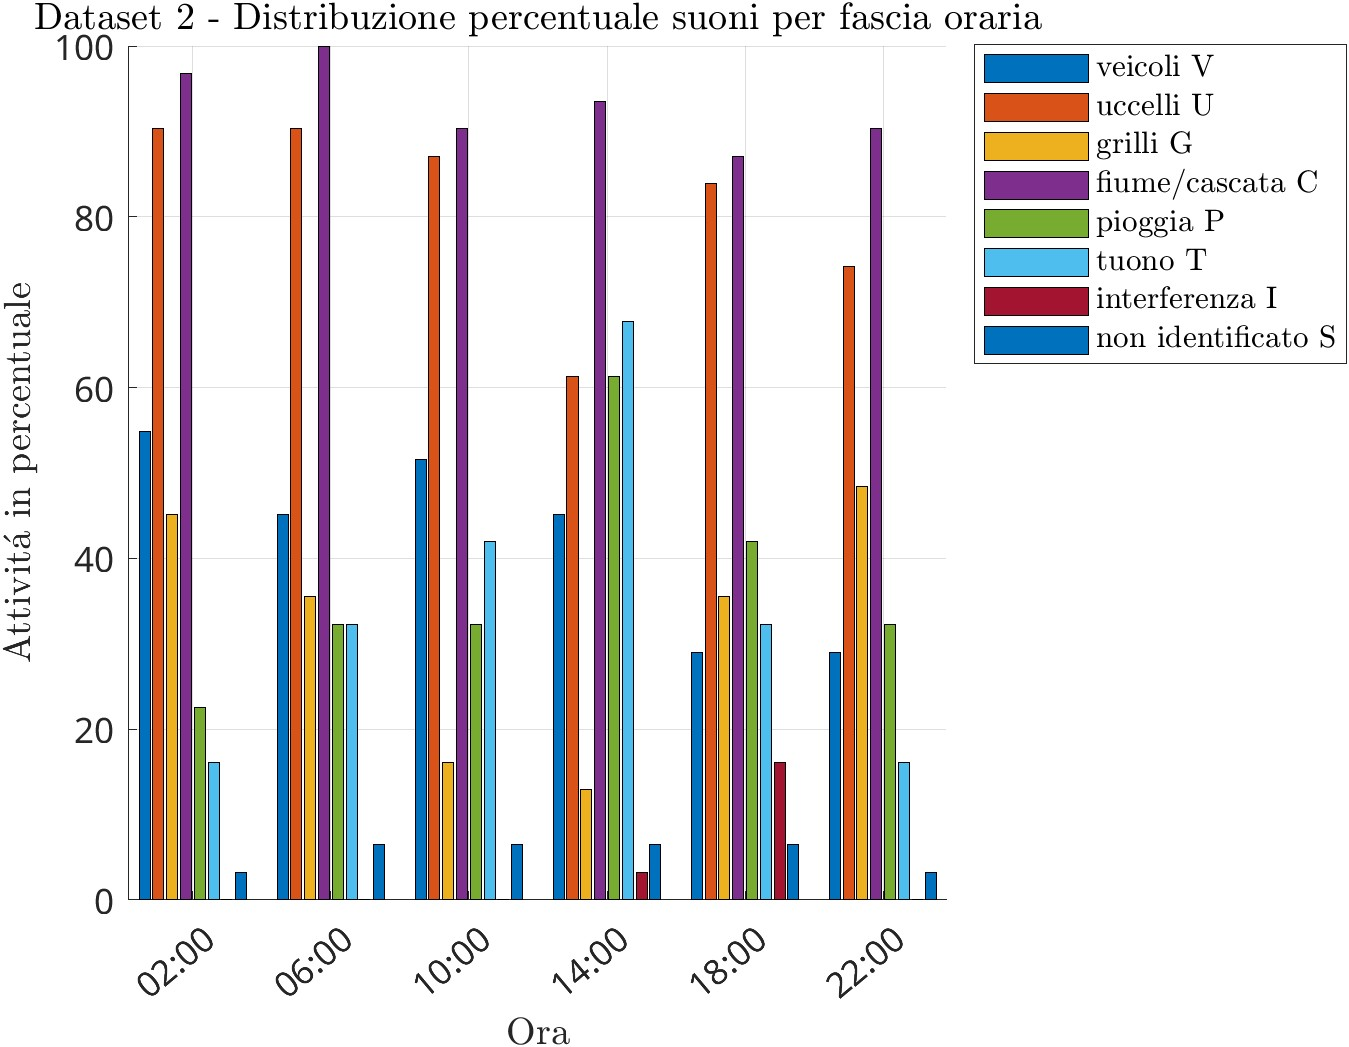
\includegraphics[width=0.9\textwidth]{img/cap3-dataset1.jpg}
	\caption{Esposizione della presenza sonora in percentuale per ogni suono nelle varie fasce orarie.}
	\label{fig3.1}
\end{figure}
\end{center}
\begin{center}
\begin{figure}[htp]
	\centering
	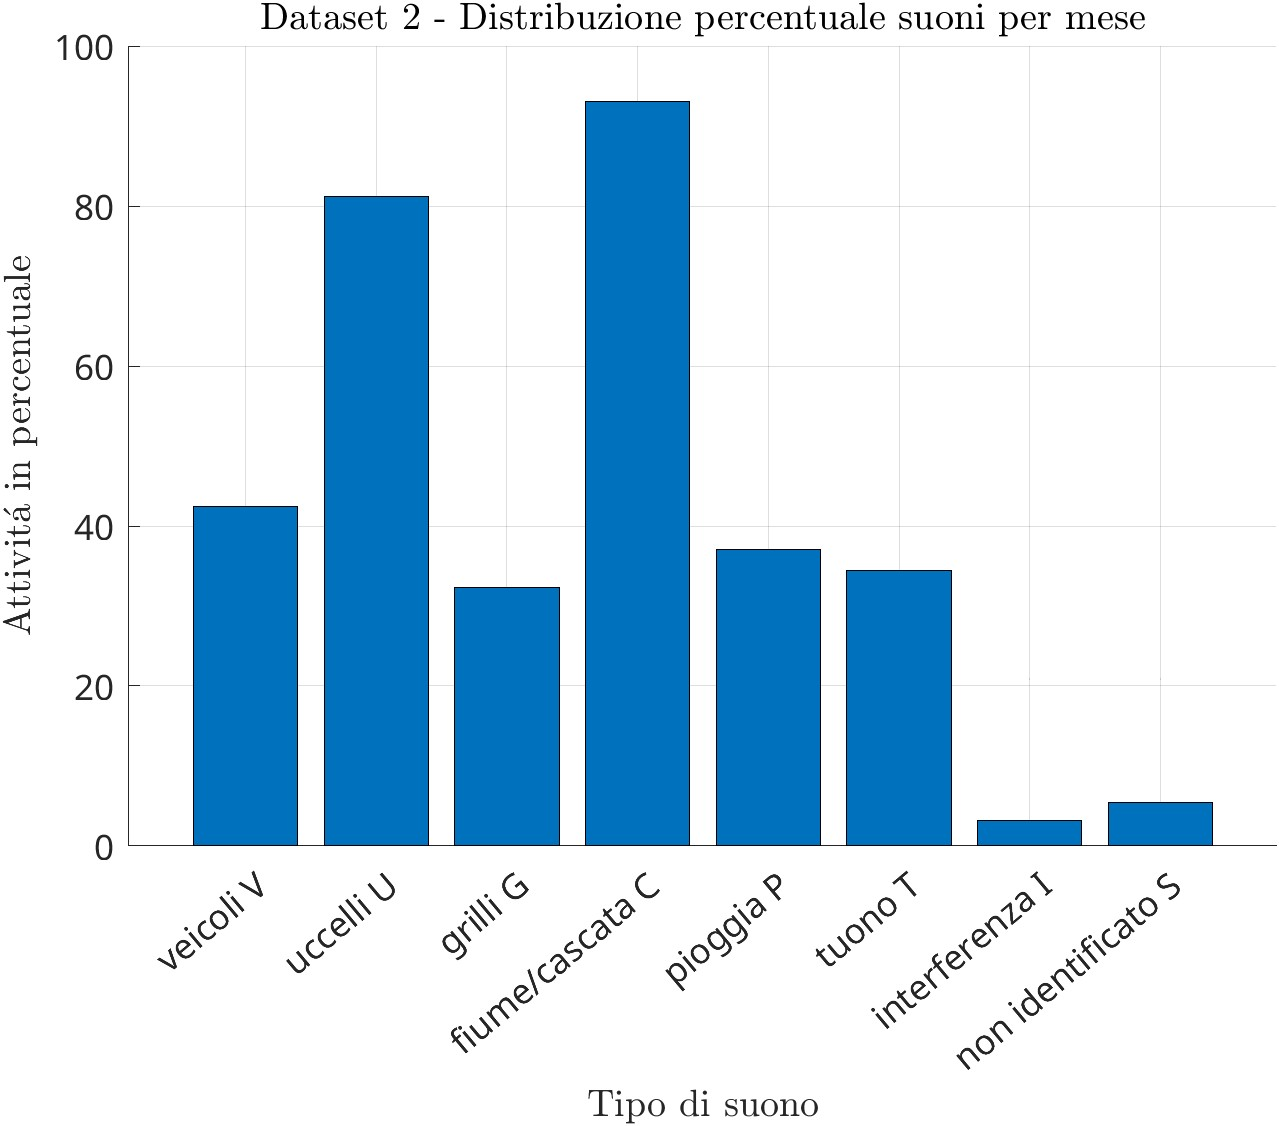
\includegraphics[width=0.8\textwidth]{img/cap3-dataset2.jpg}
	\caption{Esposizione della presenza sonora in percentuale per ogni suono in tutto il mese. Ogni suono
		presenta un percentuale di distribuzione su tutti gli audio analizzati. Si tiene in considerazione che ogni audio può contenere più suoni.}
	\label{fig3.2}
\end{figure}
\end{center}